% Turabian Formatting for Research Papers Template, 2018/08/06
%
% Developed using the turabian-formatting package (2018/08/01), available through CTAN: http://www.ctan.org/pkg/turabian-formatting
%
% Additional document class formatting options:
%
% raggedright: ragged right formatting without hyphenations
% authordate: support for the author-date citation style
% endnotes: support for endnotes



\documentclass[12pt]{turabian-researchpaper}


\usepackage[utf8]{inputenc}
\usepackage{csquotes, ellipsis,xurl,tocloft,graphicx}

% Specify paper size with geometry package
\usepackage[pass, letterpaper]{geometry}

% For citations, use the biblatex-chicago package
\usepackage{biblatex-chicago}
\addbibresource{works-cited.bib}

% Numbering the sections
\setcounter{secnumdepth}{2}
\setcounter{tocdepth}{2}
\renewcommand{\cftsecleader}{\cftdotfill{\cftdotsep}}

% Information for title page
\title{Only the Wealthy Survive}
\subtitle{How the Plan for Creating Fallout Shelters Favored White Families}
\author{Eric Altenburg}
\course{HST 415: The Nuclear Era}
\date{December 20, 2020}

\raggedright


\begin{document}

\maketitle

Coming off the heels of World War II when Eastern Europe and parts of the world were trying to recover, there was a difference in ideologies forming. The nations that were being helped by the United States adopted capitalism, whereas those under the Soviet Union employed the communist methodology. Capitalism versus communism is what initiated the Cold War with the United States and the Soviet Union being the two leading actors. Shortly thereafter, the Soviet Union developed and successfully tested their own nuclear weapons giving way to a new threat in the eyes of the United States; there was now another nuclear superpower. Knowing that the United States was no longer in nuclear control led to a growing anxiety among its citizens with fears of a nuclear war coming to cities where millions lived. Further adding to this stress was a film called "Duck and Cover" released by the Civil Defense Firm which depicted what to do in the event of a nuclear explosion. With the nation on edge in fear of a nuclear war breaking out, tensions rose once more with the Red Scare and McCarthyism—a movement to oust communists in the United States through accusations without a proper regard for any evidence. Therefore, with the nation whose stress levels were at an all time high, the only thing that gave them a sense of well-being and safety were fallout shelters. These locations were marked with an iconic yellow and black sign, and they were meant to provide safety for occupants from radioactive debris and fallout from a nuclear blast. However, creating these places on such short notice was difficult and expensive, so a solution was to inspect all known buildings to see if they met the requirements of a fallout shelter. But it was often the case that these buildings were constructed too long ago to adequately hold up against a nuclear blast—not that any buildings were realistically capable of withstanding such a blast—and because of this, Americans were encouraged to build their own in their backyard. This idea of having people find their own solutions causes problems, specifically this creates an issues of selectively choosing who can and cannot survive a nuclear war. While not necessarily inherently racist or biased towards one race, the distribution of the shelters was centered around areas that were found to be newer and able to withstand a blast, and they were often found in areas where the surrounding population was wealthier and had more money flowing through. Additionally, since families were encouraged to build their own bunkers and fallout shelters in the event of a nuclear explosion, this meant they were expected to be able handle the enormous upfront cost to build such a structure. Not all families in the United States had the means and extra income to afford a project like that. This preference toward wealthy families coupled with the wage gap between races in the years of the Cold War shows that while not explicitly targeting white communities to build fallout shelters, they were indirectly prioritized. 


The feeling of needing to have a fallout shelter nearby at all times was not common initially, however, after the release of Civil Defense films like "Duck and Cover," it unintentionally scared the American people into thinking they would need one. The film was released in 1952 and tells of drills and practices that should be followed in the event of a nuclear explosion that were to go off in the distance. The main character used as a means to help the children model their behavior after was Bert the Turtle who would err on the side of caution always making sure to duck and cover himself at the onset of danger \footnote{United States. Office of Civil Defense, "Duck and Cover," film, video, from Library of Congress, Motion Picture, Broadcasting And Recording Sound Division, 1951, https://www.loc.gov/item/mbrs01836081/.}. This translated well for nuclear blasts because even though someone would not necessarily survive an explosion up close, if the bomb were to go off far away, there was a chance of surviving by ducking and covering; people would likely walk away with burns or similar injuries. Another video by the Civil Defense organization was the "House in the middle" where it further showed how to survive a nuclear blast by painting a house with a fresh coat and keeping it free of loose garbage could be the difference between life and death \footnote{National Paint, Varnish, and Lacquer Association, "The House in the Middle. Second Version," 1954, video, https://www.loc.gov/item/mbrs02034317/.}. Even though the goal of these films was to warn, by showing them, it resulted in increased anxiety for the citizens of the United States; the threat of nuclear war felt more real. 


In another attempt to make this topic more digestible for children, shelters located at schools were often modified to feel more welcoming. The article "How 'Duck-and-Cover' Drills Channeled America's Cold War Anxiety" shows how the aforementioned film actually ended up becoming a driving factor in the fears of the time. It tells of JoAnne Brown's experiences saying, "teachers in Detroit sang songs, told stories and played records while children were in the 'refuge area,' while a teacher in Newton, Massachusetts, decorated the school bomb shelter as a 'reading den'" \footnote{Sarah Pruitt, "How 'Duck-and-Cover' Drills Channeled America's Cold War Anxiety," \textit{History}, March 26, 2019, https://www.history.com/news/duck-cover-drills-cold-war-arms-race.}. This is a perfect example of how the teachers at the time were trying to incorporate nuclear war into the everyday lives of their students; a place to go when a bomb goes off can also be a place where they can read, sing, and have fun; it makes the idea easier to understand. However, it is important to note that there was also another side to this thinking. Further on in the article, Professor Wellerstein states that the juxtaposition of the imagery of reading a book in a refuge area meant for when an atomic bomb goes off showed that people knew it was not going to work \footnote{Pruitt, "Cold War Anxiety."}. Decorating the walls of the bomb shelter reduced the overall weight the facility carried, now the facility seemed childish and not capable of withstanding a nuclear war. They felt that there was no hope if a nuclear war started, the most they could do was simply duck and cover themselves hoping that they were far enough away from the blast to survive.

Even though, a portion of the population felt uneasy about these shelters, the government knew that it was the only viable way of providing civil defense, and therefore, continued to push for their construction. President Eisenhower appointed the Gaither Committee to research into the ways the United States could better prepare itself in the event of a nuclear attack. Their report pointed out various ways in which the country fell short in protecting its citizens and that more funds should be put toward strengthening the nation's military defense. With regard to protecting the citizens on a massive scale, it recommended, "a nationwide fallout shelter program to protect the civilian population," and while not immediately pushing for them to be built, they said, "it appears prudent to carry out promptly a research and development program for such blast shelters since we must be in a position to move rapidly into construction should the need for them become evident" \footnote{Security Resource Panel of the Science Advisory Committee, "Deterrence \& Survival in the Nuclear Age (Gaither Report)" (Executive Office of the President 1957), 8, https://nsarchive2.gwu.edu//NSAEBB/NSAEBB139/nitze02.pdf.}. While proposing a shelter program, they later stated the reason for not pushing the immediate deployment of this job is due to cost, after doing the calculations, it was found that in order to put in effect measures that include "fallout shelter program including R\&D for blast shelters," it would cost \$22.5 billion \footnote{Security Resource Panel of the Science Advisory Committee, "Deterrence \& Survival in the Nuclear Age," 24.}. This staggering price was not something that could easily be allocated or warrant such an allocation because up until this point, there were only two nuclear bombs to ever be used in a war—both at the hands of the United States. Because of this, the budget that would eventually pass through congress fell short significantly at \$207.6 million. With this small budget, new plans were made and a new direction had to be taken if the American people were to be prepared and safe in the event of a nuclear explosion.

President John F. Kennedy announced in 1961 a plan to survey existing buildings to be marked as a fallout shelter, this would later be called the National Fallout Shelter Survey Program. Local architects were hired to inspect existing buildings to see if they met the minimum requirements to be considered a fallout shelter. The main unit of measurement for these buildings was its protection factor which was to be individually calculated for each shelter. A protection factor of 100 would mean that while in the shelter, the individual would receive $\frac{1}{100}$ the amount of radiation as opposed to being outside in the fallout. These factors would range from 20 to 100 with the former likely not being designated as a public shelter. If its protection factor was sufficient, then it would be marked as a public shelter and two-weeks worth of food, water, and other supplies was to be sent to it. But if it was not satisfactory, then the feasibility and cost had to be determined for upgrading a building to meet the requirements. The error with this program did not originate in the survey, but instead with the reliance on the local civil defense agencies tended to fall short. They would be responsible for all of the upkeep of the shelters after establishing them; this includes, marking and stocking the shelters, performing annual checkups to ensure proper guidelines are being met, and updating local shelter use plans. \footnote{Kathryn Plimpton, "The Forgotten Cold War: The National Fallout Shelter Survey and the Establishment of Public Shelters" (MS thesis, University of Colorado at Denver, 2000), 22, PQDT Open.}.

The group in charge of the approved public shelters before handing them off to local civil defense agencies was the Office of Civil Defense. These regional civil defense offices would communicate with the local civil defense to coordinate the drop-off of supplies, but once the shipment left their hands, they felt that they were no longer obligated to help the shelter anymore. This is the downfall to the National Fallout Shelter Survey. Although the shipment was on its way to the local civil defense groups, the issue then turns into attempting to distribute them to each shelter. Two-weeks worth of supplies for one shelter is not easy to move with a small group of civil defense workers, so to have all of the surrounding shelters' supplies in the same shipment makes the process that much more difficult. Not only were these local civil defense groups lacking in workforce, but they were also responsible for locating a warehouse to store these supplies while the allocations for each shelter is being calculated. After the shipments were divided up for each shelter, then they had to plan the method of shipping for these shelters.

Another area of concern with the National Fallout Shelter Survey project was again with the local civil defense groups' abilities to create and coordinate local shelter use protocols. The Office of Civil Defense thought it would be best for the local offices to handle these shelters because they would be able to determine a personalized plan for each community as one blanket-protocol for all the shelters would likely not succeed; a plan for New York City should be different than one for a rural town. Using maps of day and night populations along with the locations of the potential shelters, the local offices could then make a plan that would fit each town individually. However, this did not work as intended because many of these local offices did not have the workers who were properly trained to handle such planning. \footnote{Kathryn Plimpton, "The Forgotten Cold War," 25.} One such example of this failure in designing a plan happened in Denver, Colorado:

	\begin{quotation}
		The 1963 plan gave detailed descriptions of the types of sirens and warnings that might be heard before an attack. the plan then skipped the emergence of survivors from their fallout shelters, the continuity of city government, the restoration of municipal services, and how aid would be given to those injured during or after the attack. Nowhere in the plan was there a discussion of how the public would locate the nearest shelter or what to do if shelters were full or if there was no shelter nearby. There were no maps of shelters or discussions regarding the number of people who might be found without protection. \footnote{Kathryn Plimpton, "The Forgotten Cold War," 36.}
	\end{quotation}

This is the epitome of the worst case scenario, and while this was only one yearly plan the local offices came up with, the next was also littered with similar mistakes and calculation errors with the amount of people who could actually be placed in a shelter. Additionally, these plans were never actually released to the public, this means that for two years after the buildings were inspected and marked by the Office of Civil Duties, civilians did not know how to access or use the facilities in the event of a nuclear detonation.

Prior to the aforementioned issues of a government run program to create fallout shelters nationwide, President John F. Kennedy stated that families should begin to look into a means of making their own shelters in the meantime. While the statement might have been directed to the entire nation, it only applied to a select population of the American people. The issue with families building their own bunkers without the help of the government is the cost, since it is privatized, there is no set limit as to how much a bunker would have cost. And the range between the specifications that each private bunker had ranged significantly depending on the upfront cost families were willing to pay. For example, a video released by the Office of Civil and Defense Mobilization titled "Walk Builds a Family Fallout Shelter" goes over the process of building a shelter under a home in its basement. Its materials are mainly brick—with a fresh coat of paint of course—but this would likely not be sufficient for a shelter \footnote{United States. Office of Civil Defense, "Walt Builds a Family Fallout Shelter," film, video, Records of the Federal Emergency Management Agency, Record Group 311, 1960, https://www.docsteach.org/documents/document/walt-builds-a-family-fallout-shelter.}. Expanding on this, in 1961, a story on the front page of the Washington Post told that most of the shelters would be a little more than "cold, unpleasant cellar space, with bad ventilation and even worse sanitation" \footnote{Robert Klara, "Nuclear Fallout Shelters Were Never Going to Work," \textit{History}, October 16, 2017, https://www.history.com/news/nuclear-fallout-shelters-were-never-going-to-work.}. Another type of shelter that would provide similar terrible conditions for families involved using a big enough pipe to fit three people. This was one of the most cost effective options at \textasciitilde \$150. This would not provide enough shelter, protection, and comfort for the family though as they would need to remain in the pipe for up to two weeks until the fallout stops coming down. On the other hand, a nicer end shelter called a Kidde Kokoon went for \textasciitilde \$3,000 and this provided an ample amount of space for a family of four with enough room to store two weeks worth of supplies. Obviously out of the two types of shelters the latter is preferred as it has the best chance of keeping a family safe from fallout, however, not every family at the time could afford such a shelter. When the president made that announcement, it realistically only pertained to the wealthy white families who had the expendable income to build one. The wage gap based on race was a very real issue at the time of the cold war, see Figure \ref{WealthAvg}. In 1963, the average income for a white family was \$140,633 whereas a nonwhite family made \$19,504. For a shelter that cost \textasciitilde \$3,000, a white family was more likely to be able to afford it as after purchasing, they would still have at least \$137,633 but a nonwhite family would have \$16,504. Also, his price does not include any preparations that would have to be made to the yard prior to installation so the upfront cost is likely to be even higher. With only a specific population of individuals who can afford shelters that would actually provide adequate protection, those who could not afford them were most likely holding out for the government shelter program. However, as it was previously mentioned, towns would go years without any solid plan for gaining access to such shelters thus leaving them completely vulnerable while the white families who could afford a shelter had a backup plan.

\begin{figure}[!h]
    \centering
    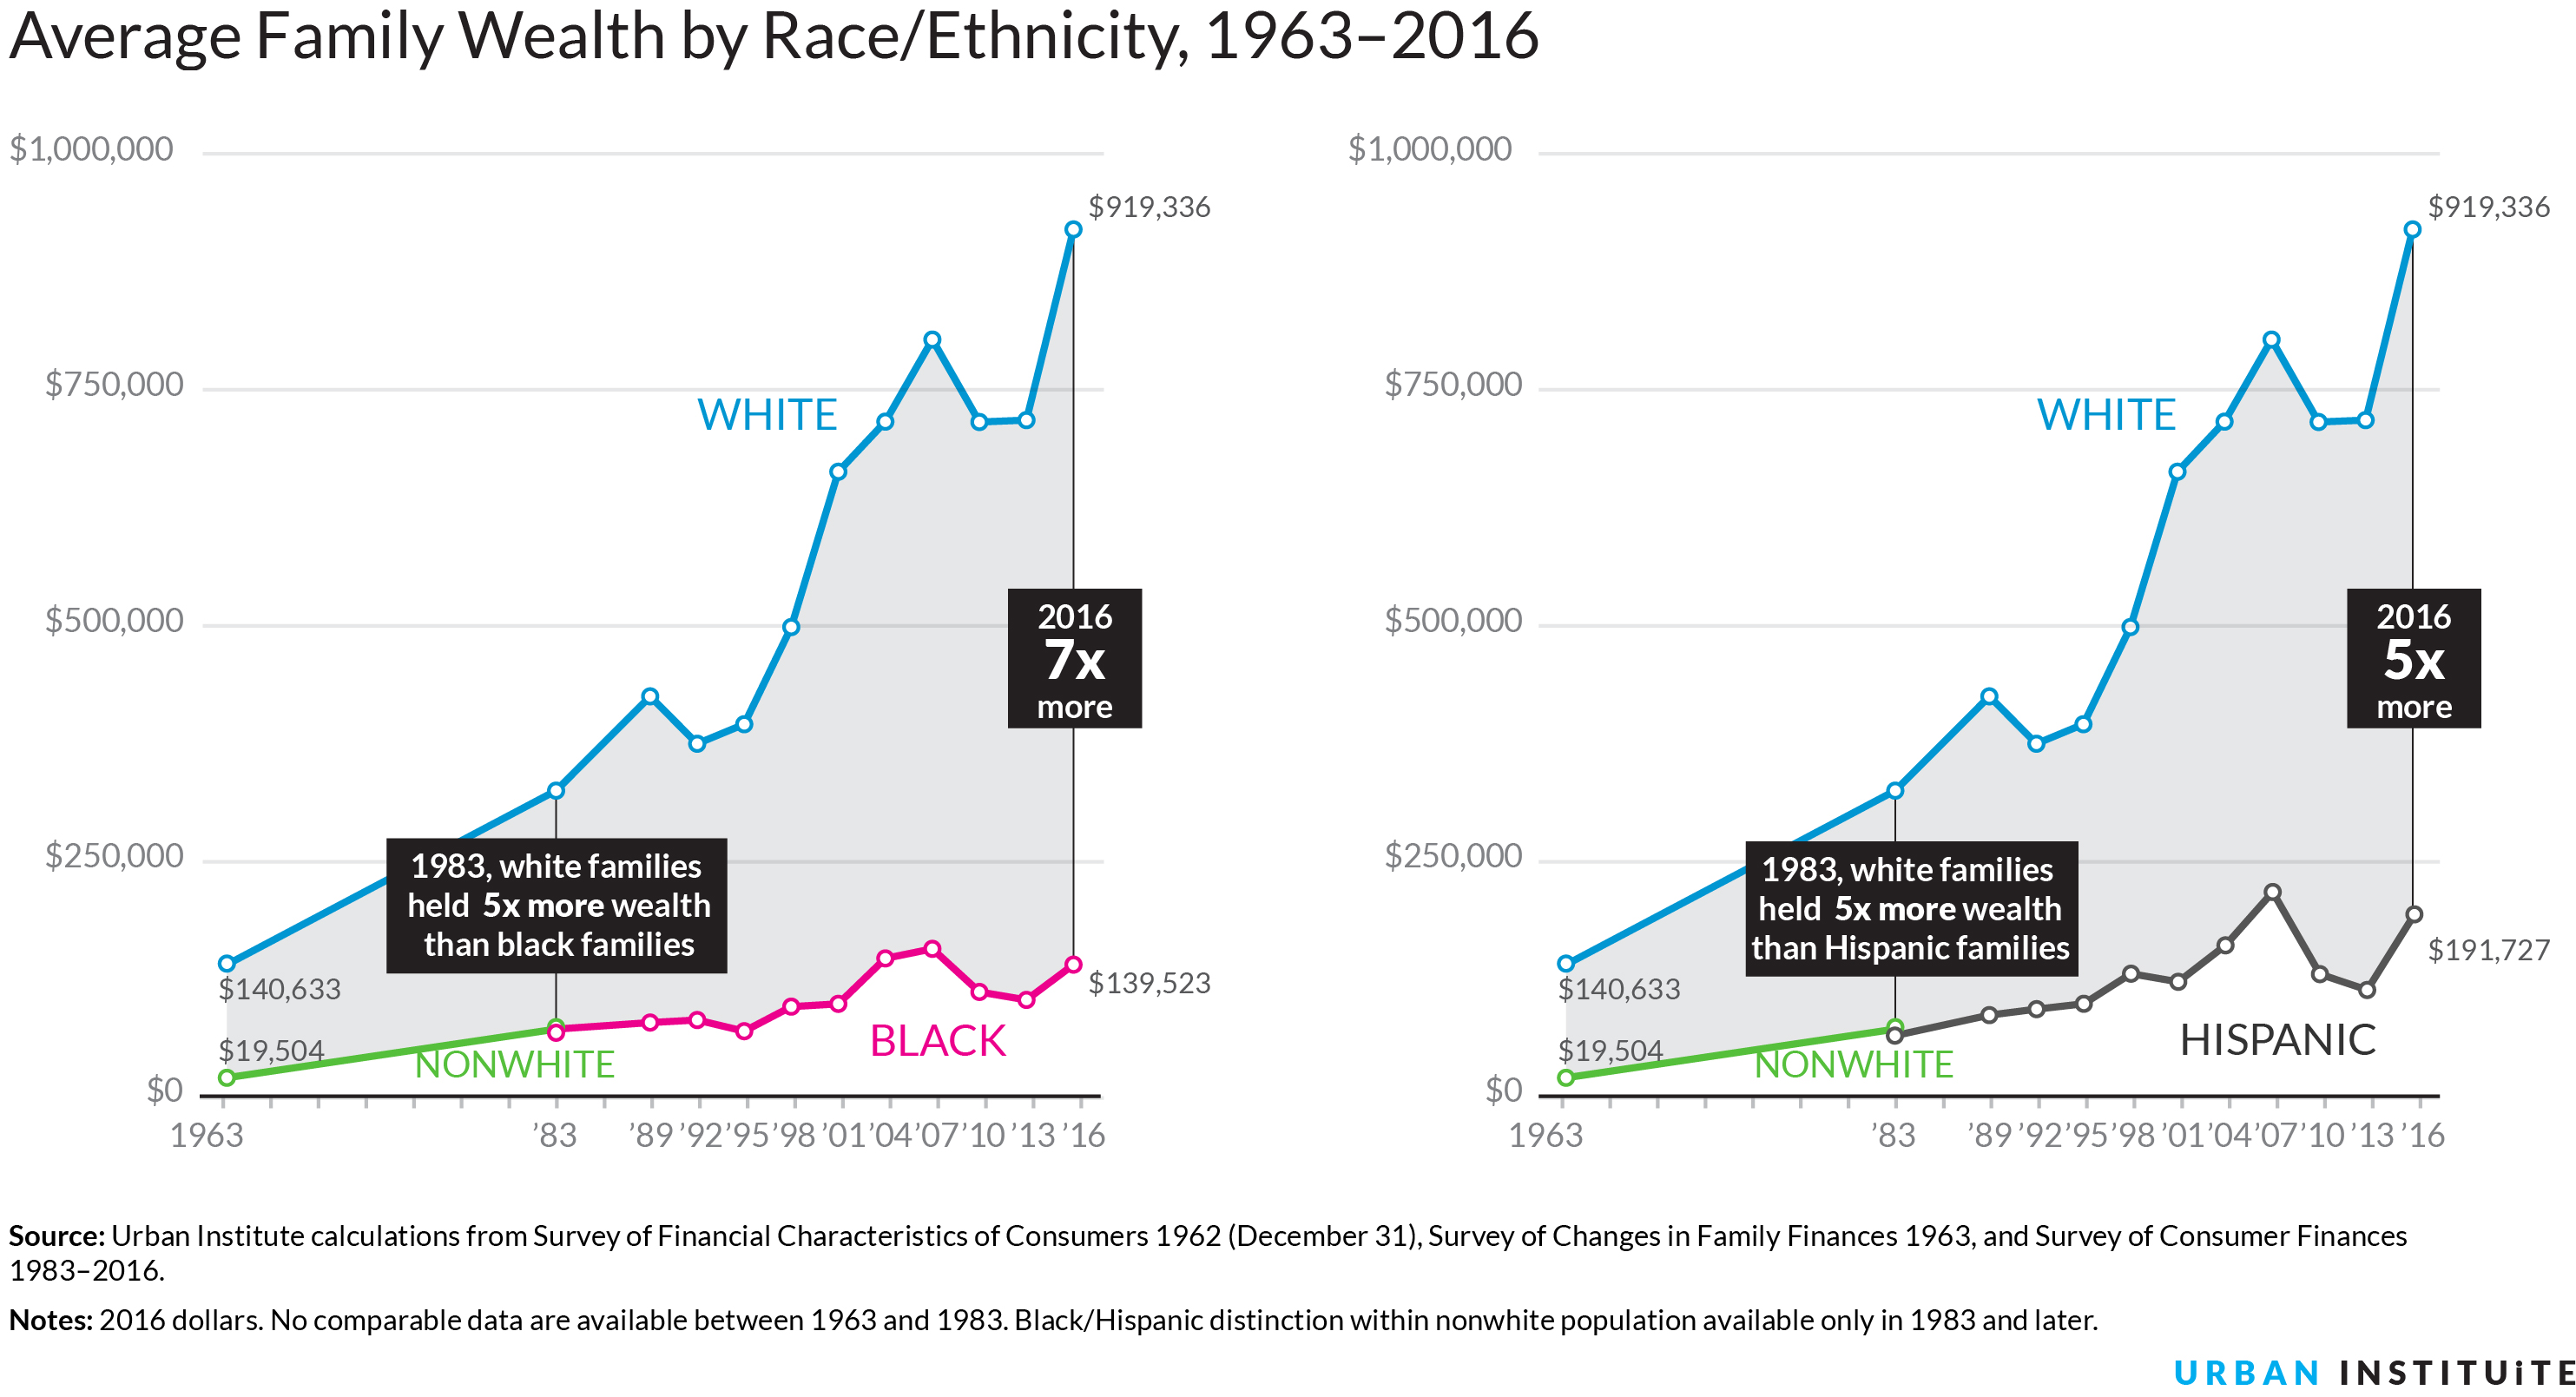
\includegraphics[scale=0.6]{images/WealthByRace-avg.jpeg}
    \caption{This shows the disparity between the average wages of white and nonwhite families.}
    \label{WealthAvg}
\end{figure}



The popularity of the fallout shelter rising exponentially over the years of the Cold War due to anxiety among the American people spiking from films like "Duck and Cover," "The House in the Middle," and "Walt Builds a Family Fallout Shelter." Adopting the safety procedures in the event of everyday life with school children made nuclear war feel as if it were inevitable, and that it would live with them for years to come. As a means of helping the public indirectly cope with this, fallout shelters were seen as a viable solution to civil defense, however, after the Gaither Committee researched and discovered the immense upfront cost of a proper nationwide program would be, other solutions were sought out. Before deploying the National Fallout Shelter Survey, citizens were encouraged to go out and buy their own shelters as a means of guaranteeing their own safety, however, not everyone in the country had the financial means of experiencing this safety. White families were put at an advantage as their average income was seven times that of a nonwhite family. By encouraging these private shelters, white families were indirectly prioritized and given the opportunity at survival in the case of a nuclear war, and for the many nonwhite families, they had to wait for the unreliable public shelters. The same shelters that were not run properly by local civil defense groups and as a result, the families were put in danger for every passing day they did not have access to a shelter.





\newpage

\begin{thebibliography}{100}
	\bibitem{5}{Kathryn Plimpton. ”The Forgotten Cold War: The National Fallout Shelter Survey and the Establishment of Public Shelters.” MS thesis, University of Colorado at Denver, 2000. PQDT Open.}
	\bibitem{2}{National Paint, Varnish, and Lacquer Association. ”The House in the Middle. Second Version.” 1954. Video. https://www.loc.gov/item/mbrs02034317/.}
	\bibitem{7}{Robert Klara. ”Nuclear Fallout Shelters Were Never Going to Work.” \textit{History}, October 16, 2017. https://www.history.com/news/nuclear-fallout-shelters-were-never-going-to-work.}
	\bibitem{3}{Sarah Pruitt. ”How ’Duck-and-Cover’ Drills Channeled America’s Cold War Anxiety.” \textit{History}, March 26, 2019. https://www.history.com/news/duck-cover-drills-cold-war-arms-race.}
	\bibitem{4}{Security Resource Panel of the Science Advisory Committee. ”Deterrence \& Survival in the Nuclear Age (Gaither Report).” Executive Office of the President, 1957. https://nsarchive2.gwu.edu//NSAEBB/NSAEBB139/nitze02.pdf.}
	\bibitem{8}{Signe-Mary McKernan, et al. "Nine Charts About Wealth Inequality in America (Updated)." Last Modified October 5, 2017. https://apps.urban.org/features/wealth-inequality-charts/.}
	\bibitem{1}{United States. Office of Civil Defense. ”Duck and Cover.” Film, video. From Library of Congress, Motion Picture, Broadcasting And Recording Sound Division, 1951. https://www.loc.gov/item/mbrs01836081/.}
	\bibitem{6}{United States. Office of Civil Defense. ”Walt Builds a Family Fallout Shelter.” Film, video. Records of the Federal Emergency Management Agency, Record Group 311, 1960. https://www.docsteach.org/documents/document/walt-builds-a-family-fallout-shelter.}
\end{thebibliography}

\end{document}